\scanpage{63}
\mspage{3.}
% archive foliation: 62
d'application du thme de spécialisation \deleted{\unsure{du groupe}}
des revêtts tame \ldots

Lorsque $X$ n'est pas normal, on utilise la descente \ldots\ À détailler.
\margin{\figure{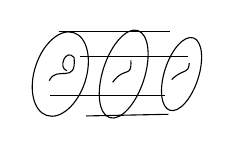
\begin{tikzpicture}[scale=.7]
\draw[rotate around={-18:(0,0)}] (0,0) ellipse (.47 and .79);
\draw[rotate around={-18:(1.15,0)}] (1.15,0) ellipse (.38 and .83);
\draw[rotate around={-18:(2.2,0)}] (2.2,0) ellipse (.31 and .69);
\draw (-.03,.78)--(1.99,.78);
\draw (.36,.32)--(2.32,.32);
\draw (-.18,-.39)--(1.9,-.39);
\draw (.47,-.76)--(1.96,-.73);
\draw (-.20,-.12)..controls (-.07,.17) and (.3,-.2)..(.25,.3)
..controls (.10,.48) and (-.05,.11)..(.12,.06);
\draw (.95,-.15)..controls (1.17,.15) and (1.30,-.08)..(1.28,.25);
\draw (2.02,-.10)..controls (2.25,.12) and (2.32,-.02)..(2.34,.2);
\end{tikzpicture}}}

\uline{Corollaire} \deleted{\unsure{Soit}}
Soit $U$ de type fini sur $k$, $Y$
\deleted{\unsure{quelconque}}
(quelc. sur $k$) \inserted{$y\in Y$}
$R$ un revêtement étale \inserted{gal} de $U\times_k Y$,
de groupe $\Gamma$ premier à $p$.
\deleted{\unsure{Alors $U$}}
Si $R_y$ est un rev. géom trivial,
Alors $R$ est, en dessus d'un voisinage de
\deleted{\unsure{$U(k)$}}
$y$, l'image \unsure{directe|inverse} d'un rev étale d'un tel voisinage.

\uline{Cor.} Soient $X',X''$ propres sur $k$,
$Z'$ ($Z''$) des parties fermées, \deleted{\unsure{alors}} écrivons
\deleted{\unsure{Soit}}
$X=X'\times X''$, $Z=Z'\times X''\cup X'\times Z''$,
enfin considérons les grps
$\pi_1^t(X';Z',x')$, $\pi_1^t(X'';Z'';x'')$ et
$\pi_1^t(X;\deleted{X'\times X''}Z,x)$,
\deleted{Alors} soient $\pi,\pi',\pi''$.
Alors
\[
\deleted{\pi_1^t(X)}\quad \pi\longrightarrow\pi'\times\pi''
\]
est un \uline{\unsure{isomorphisme}}.

\uline{Cor.} Soient $X,Y$ de type fini sur $k$.
Considérons $\pi'_1(X)$ et $\pi'_1(Y)$,
\inserted{$\pi'_1(X\times Y)$}
[rev. étales premiers à la car].
Alors
\[
\pi'_1(X\times Y)\simeq\pi'_1(X)\times\pi'_1(Y).
\]
